% =================================================================================================
% File:			content_files.tex
% Description:	Defiinisce i capitoli presenti nel documento
% Created:		2015-04-21
% Author:		Tesser Paolo
% Email:		tesser.paolo@mashup-unipd.it
% =================================================================================================
% Modification History:
% Version		Modifier Date		Change											Author
% 0.0.1 		2015-04-21 			creazione struttura								Tesser Paolo
% =================================================================================================
%

% DEFINIZIONE FUNZIONE GLOSSARIO
% Questa funzione si occupa di disegnare la lettera per ogni sezione del glossario

\newcommand{\letteraGlossario}[1] { 
  \phantomsection
  \vspace{11pt}
  \textbf{\huge{#1} }
  \\
  % Traccia linea orizzontale
  \rule[0.3pt]{\linewidth}{0.4pt} \\
} 

% DEFINIZIONE DEI CONTENUTI DEL DOCUMENTO

% =================================================================================================
% File:			introduzione.tex
% Description:	Defiinisce la sezione relativa al capitolo introduttivo del documento
% Created:		2015-04-21
% Author:		Tesser Paolo
% Email:		tesser.paolo@mashup-unipd.it
% =================================================================================================
% Modification History:
% Version		Modifier Date		Change											Author
% 0.0.1 		2015-04-21 			creato scheletro doc e primo abbozzo			Tesser Paolo
% =================================================================================================
%

% CONTENUTO DEL CAPITOLO

\section{Introduzione} % (fold)
\label{sec:introduzione}
	\subsection{Scopo del documento} % (fold)
	\label{sub:scopo_del_documento}
	Questo documento ha come scopo quello di illustrare le procedure da seguire per svolgere le operazioni previste per l'utente amministratore relative al prodotto \projectName. All'utilizzatore non è chiesta nessuna particolare conoscenza informatica. Alcune operazioni richiedono però che esso abbia dimestichezza con i social network e con le possibilità che offrono.
	% subsection scopo_del_documento (end)

	\subsection{Scopo del prodotto} % (fold)
	\label{sub:scopo_del_prodotto}
	\productScope
	% subsection scopo_del_prodotto (end)

	\subsection{Prerequisiti} % (fold)
	\label{sub:prerequisiti}
	TODO (prendere spunto dagli Steakholders)
	% subsection prerequisiti (end)

	\subsection{Problemi e malfunzionamenti} % (fold)
	\label{sub:problemi_e_malfunzionamenti}
	TODO (prendere spunto dagli Steakholders)
	% subsection problemi_e_malfunzionamenti (end)

	\subsection{Glossario} % (fold)
	\label{sub:glossario}
	TODO (forse servirà inserire il glossario in appendice in quanto agli utenti non viene fornito l'altro Glossario) \newline
	\glossarioDesc
	% subsection glossario (end)

	\subsection{Riferimenti} % (fold)
	\label{sub:riferimenti}
		\subsubsection{Normativi} % (fold)
		\label{ssub:normativi}
			\begin{itemize}
				\item \textbf{Analisi dei Requisiti}: \docNameVersionAdR
				\item \textbf{Specifica Tecnica}: \docNameVersionST
			\end{itemize}
		% subsubsection normativi (end)

		\subsubsection{Informativi} % (fold)
		\label{ssub:informativi}
			\begin{itemize}
				\item \textbf{TODO}: TODO;
			\end{itemize}
		% subsubsection informativi (end)
	% subsection riferimenti (end)
% section introduzione (end)
% section introduzione (end) \newpage \clearpage
% =================================================================================================
% File:			gest_recipe.tex
% Description:	Defiinisce la sezione relativa ad un capitolo del documento
% Created:		2015-04-21
% Author:		Tesser Paolo
% Email:		tesser.paolo@mashup-unipd.it
% =================================================================================================
% Modification History:
% Version		Modifier Date		Change											Author
% 0.0.1 		2015-04-21 			creato scheletro doc							Tesser Paolo
% =================================================================================================
%

% CONTENUTO DEL CAPITOLO
\section{Gestione delle Recipe} % (fold)
\label{sec:gestione_delle_recipe}


	\subsection{Contenuti Sezione} % (fold)
	\label{sub:contenuti_sezione}
		All'utente amministratore sono concessi permessi di modifica e gestione delle recipe\gloss{}.
		La gestione prevede:
		\begin{itemize}
			\item Aggiunta di una nuova recipe\gloss{};
			\item Eliminazione di una o più recipe\gloss{};
			\item Visualizzazione classifica delle recipe\gloss{};
		\end{itemize}


	\subsection{Aggiunta di una nuova recipe}
		Dal menu principale situato nella dashboard\gloss{} del sistema è possibile visualizzare l'elenco delle recipe\gloss{} premendo sull'apposito pulsante \textbf{Recipe}.\newline
		Tramite il pulsante \textbf{New Recipe} è possibile accedere alla nuova pagina (Figura: \ref{fig:aggiunta_nuova_recipe}) per l'inserimento guidato di nuove recipe\gloss{}.
		\begin{figure}[H]
			\centering
			\centerline{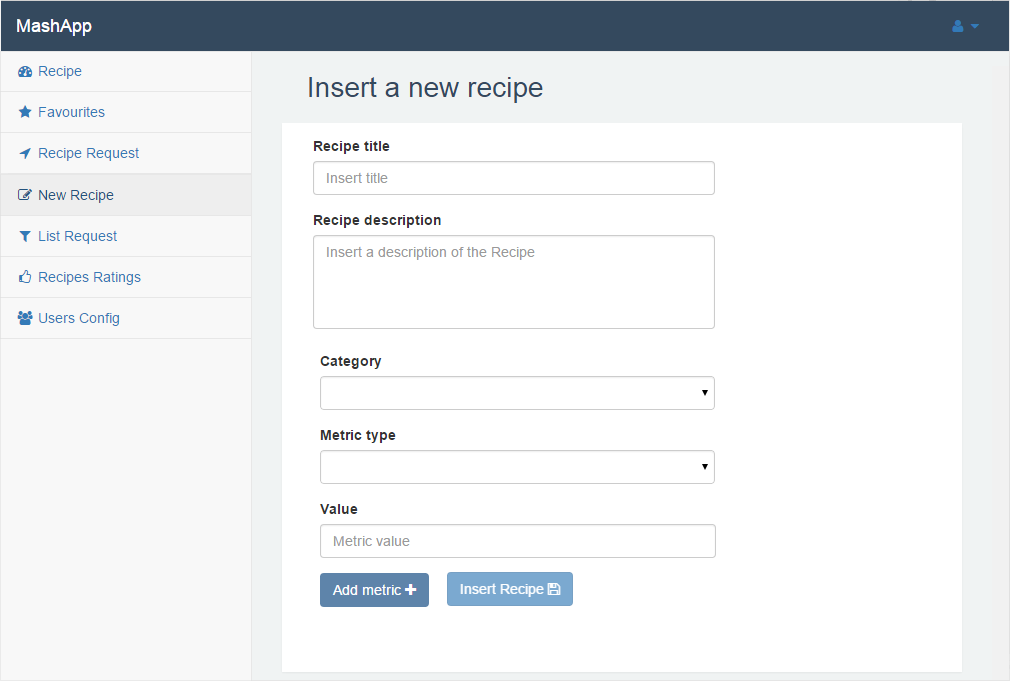
\includegraphics[width=14cm]{images/nuova_ricetta.png}}
			\caption{Aggiunta nuova recipe}
			\label{fig:aggiunta_nuova_recipe}
		\end{figure}
		Per aggiungere una nuova nuova recipe\gloss{} è necessario compilare tutti i campi del form\gloss{} (Figura: \ref{fig:aggiunta_nuova_recipe}) con i seguenti dati:
		\begin{itemize}
			\item Nome della recipe;
			\item Descrizione della recipe;
			\item Parametri relativi alla recipe dipendenti dal/dai social network di interesse;
		\end{itemize}
		È possibile selezionare uno o più social network e uno o più parametri per ciascuna selezione.\newline
		Al termine della procedura guidata è necessario premere il pulsante di \textbf{Insert Recipe} per salvare le modifiche ed aggiungere così la recipe\gloss{} al sistema.
	% END


	\subsection{Eliminazione Recipe}
		L'amministratore può eliminare una recipe\gloss{} e tutti i dati ad essa associati dal sistema.\newline
		Per accedere all'area dedicata della dashboard\gloss{} si deve premere sul pulsante \textbf{Recipe}\gloss{}. Dall'elenco delle recipe\gloss{} (Figura: \ref{fig:dashboard}) è disponibile il pulsante \textbf{Delete recipe}.
		L'eliminazione della recipe è istantanea si può così procedere ad una nuova operazione.
	% END

	
	\subsection{Visualizzazione classifica recipe}
		L'utente amministratore può visualizzare la classifica (Figura: \ref{fig:votazioni_ricette}) delle recipe\gloss{} in ordine dalla più apprezzata alla meno apprezzata.\newline
		Per accedere alla sezione è richiesto di premere l'apposito pulsante \textbf{Recipes Ratings} dal menu principale nella dashboard\gloss{}.\newline
		\begin{figure}[H]
			\centering
			\centerline{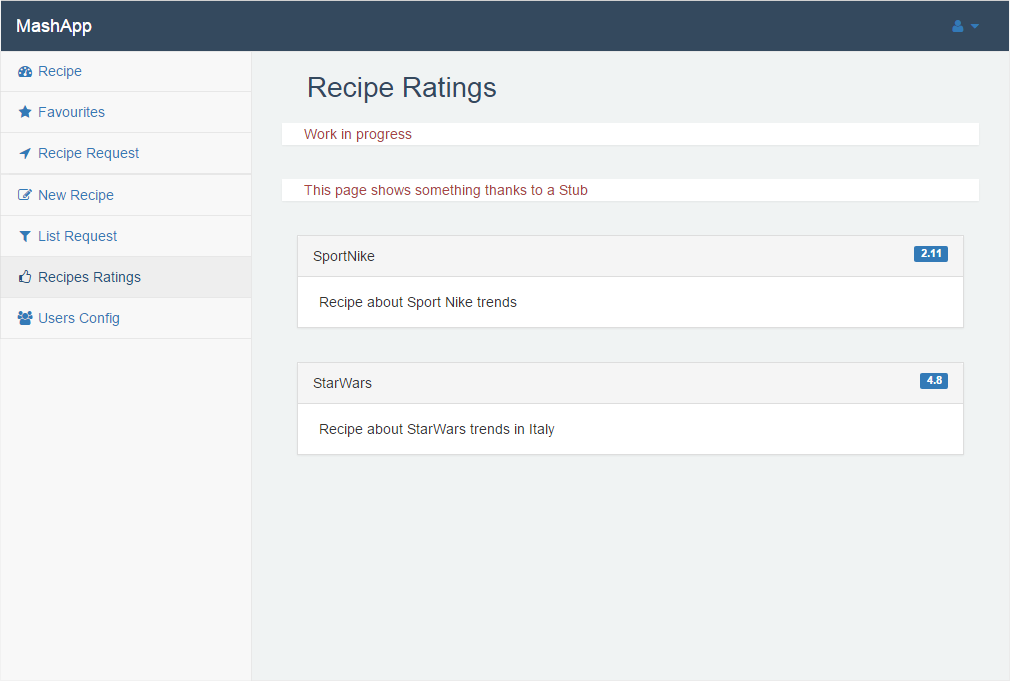
\includegraphics[width=14cm]{images/votazioni_ricette.png}}
			\caption{Punteggi recipes}
			\label{fig:votazioni_ricette}
		\end{figure}
		Nel caso in cui nessun utente abbia ancora dato un giudizio sulle recipe presenti nel sistema, la classifica risulterà vuota.\newline
		Un messaggio avviserà l'utente amministratore se questa situazione dovesse verificarsi.
	% END


% section Gestione delle Recipe (end) \newpage \clearpage
% =================================================================================================
% File:			amm_utenti.tex
% Description:	Defiinisce la sezione relativa ad un capitolo del documento
% Created:		2015-04-21
% Author:		Tesser Paolo
% Email:		tesser.paolo@mashup-unipd.it
% =================================================================================================
% Modification History:
% Version		Modifier Date		Change											Author
% 0.0.1 		2015-04-21 			creato scheletro doc							Tesser Paolo
% =================================================================================================
%

% CONTENUTO DEL CAPITOLO
\section{Gestione degli utenti} % (fold)
\label{sec:gestione_utenti}
	

	\subsection{Contenuti Sezione} % (fold)
	\label{sub:contenuti_sezione}
		All'utente amministratore sono concessi permessi di gestione degli utenti.
		La gestione prevede le seguenti funzionalità:
		\begin{itemize}
			\item Visualizzazione dell'elenco di tutti utenti registrati sull'applicazione (Figura: \ref{fig:configurazione_utenti});
			\item Modifica permessi utente (Figura: \ref{fig:configurazione_utenti}, rif. 2);
			\item Eliminazione profilo utente (Figura: \ref{fig:configurazione_utenti}, rif. 3);
		\end{itemize}
		\begin{figure}[H]
			\centering
			\centerline{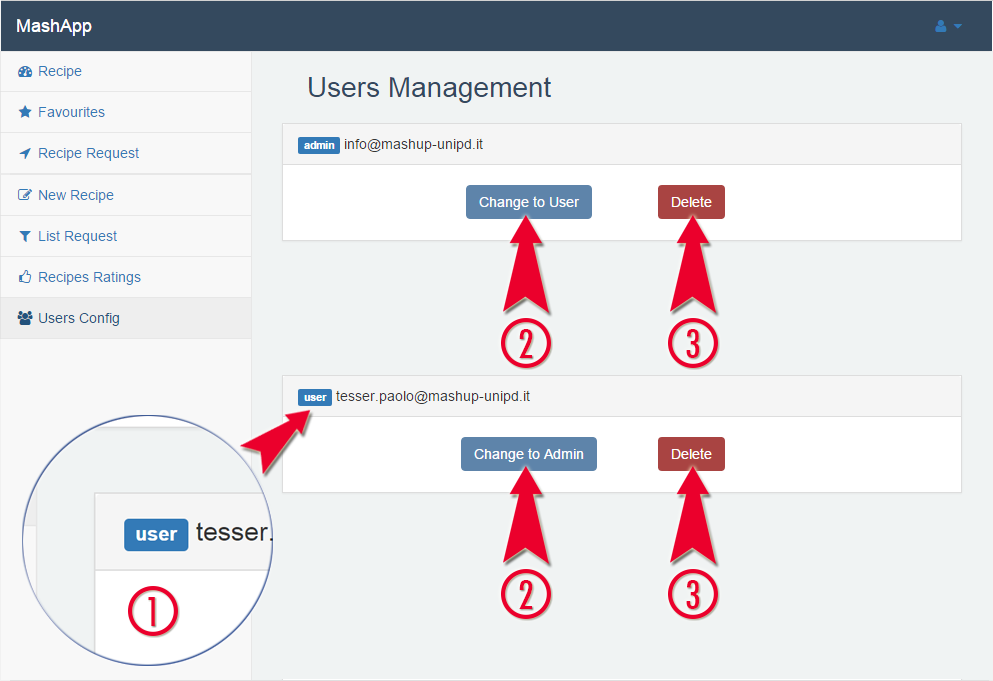
\includegraphics[width=14cm]{images/configurazione_utenti.png}}
			\caption{Gestione utenti}
			\label{fig:configurazione_utenti}
		\end{figure}
	% END

	\pagebreak
	\subsection{Visualizzazione elenco utenti}
		L'utente amministratore può visualizzare l'elenco (Figura: \ref{fig:configurazione_utenti}) di tutti gli utenti registrati nel sistema selezionando l'apposito pulsante dal menu principale (Figura: \ref{fig:menu_principale_utente}) situato nella Home Page della dashboard\gloss{} (Figura: \ref{fig:dashboard}).\newline
		In questo elenco (Figura: \ref{fig:configurazione_utenti}) è possibile visualizzare tutti i dati di ciascun utente, modificare  i suoi permessi oppure eliminare un utente, purché esso non sia un amministratore a sua volta.\newline
		L'identificazione del tipo di permessi è visualizzata per ogni singolo utente (Figura: \ref{fig:configurazione_utenti}, rif. 3).
	% END	

	
	\subsection{Modifica permessi utente}
		L'utente amministratore può abilitare i permessi di amministratore ad un utente diverso da se stesso.\newline
		Per effettuare questa operazione è necessario accedere all'elenco degli utenti (Figura: \ref{fig:configurazione_utenti}) premendo l'apposito pulsante dal menu principale di amministrazione (Figura: \ref{fig:menu_principale_utente}) dell'applicazione situato nella Home Page della dashboard (Figura: \ref{fig:dashboard}).
		La procedura prevede l'individuazione dell'utente nel sistema e la relativa pressione del pulsante \textbf{Change to admin} (Figura: \ref{fig:configurazione_utenti}, rif. 1).\newline
		Una volta effettuata la selezione è richiesto di premere il pulsante di conferma dell'operazione per rendere effettive le modifiche.
	% END

	
	\subsection{Eliminazione utente}
		L'utente amministratore può eliminare un utente diverso da se stesso dal sistema.\newline
		Per effettuare questa operazione è necessario accedere all'elenco degli utenti (Figura: \ref{fig:configurazione_utenti}) premendo l'apposito pulsante dal menu principale di amministrazione Figura: \ref{fig:menu_principale_utente}) dell'applicazione situato nella Home Page della dashboard (Figura: \ref{fig:dashboard}).
		La procedura prevede l'individuazione dell'utente nel sistema e la relativa pressione del pulsante \textbf{Delete} (Figura: \ref{fig:configurazione_utenti}, rif. 2).\newline
		Una volta effettuata la selezione è richiesto di premere il pulsante di conferma dell'operazione di eliminazione per rendere effettive le modifiche.\newline
		ATTENZIONE: l'operazione di eliminazione utente non è reversibile.
	% END
		

% section Gestione degli utenti (end) \newpage \clearpage
% =================================================================================================
% File:			gest_richieste.tex
% Description:	Defiinisce la sezione relativa ad un capitolo del documento
% Created:		2015-04-21
% Author:		Tesser Paolo
% Email:		tesser.paolo@mashup-unipd.it
% =================================================================================================
% Modification History:
% Version		Modifier Date		Change											Author
% 0.0.1 		2015-04-21 			creato scheletro doc							Tesser Paolo
% =================================================================================================
%

% CONTENUTO DEL CAPITOLO
\section{Gestione richieste recipe} % (fold)
\label{sec:gest_richieste}


	\subsection{Contenuti Sezione} % (fold)
	\label{sub:contenuti_sezione}
		L'amministratore può provvedere ad approvare o respingere l'inserimento di una nuova recipe\gloss{} proposta da un utente.\newline
		Vengono messe a disposizione dell'amministratore le seguenti funzioni:
		\begin{itemize}
			\item \textbf{See Details}: visualizza i dettagli della recipe richiesta (Figura: \ref{fig:richiesta_ricette}, rif. 1);
			\item \textbf{Discard}: disapprova la richiesta (Figura: \ref{fig:richiesta_ricette}, rif. 2);
			\item \textbf{Approve}: approva la richiesta di aggiunta (Figura: \ref{fig:richiesta_ricette}, rif. 3);
		\end{itemize}
		E' possibile visualizzare l'elenco delle recipe\gloss{} in attesa di approvazione (Figura: \ref{fig:richiesta_ricette}).
		\begin{figure}[H]
			\centering
			\centerline{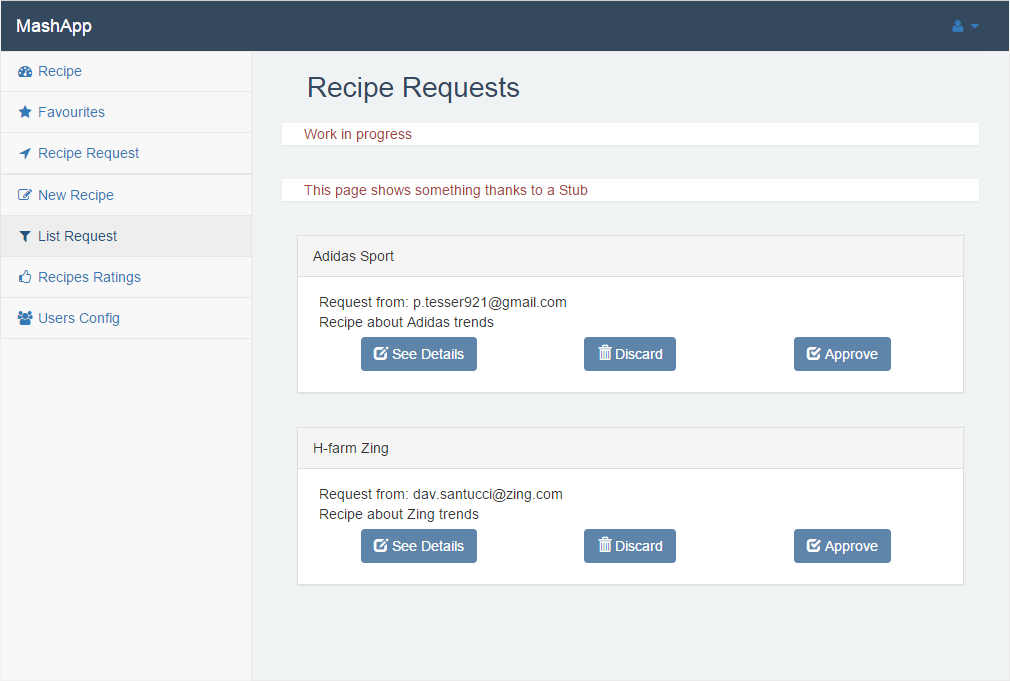
\includegraphics[width=14cm]{images/richiesta_ricette.png}}
			\caption{Approvazioni e eliminazione richieste utente}
			\label{fig:richiesta_ricette}
		\end{figure}


	\pagebreak
	\subsection{Visualizza elenco richieste}
		L'utente amministratore può visualizzare un elenco delle richieste delle recipe\gloss{} (Figura: \ref{fig:richiesta_ricette}) che sono state inviate dagli utenti normali e non ancore marcate come \textbf{chiuse}.\newline
		Per accedere all'elenco delle richieste (Figura: \ref{fig:richiesta_ricette}), selezionare l'apposito pulsante \textbf{List Request} dal menu principale della dashboard\gloss{} (Figura: \ref{fig:dashboard}).
	% END
	

	\subsection{Visualizza dettagli richiesta}
		L'utente amministratore può visualizzare tutti i dettagli di una richiesta, dopo aver premuto il pulsante \textbf{See Details} (Figura: \ref{fig:richiesta_ricette}, rif. 1) dall'elenco delle richieste.\newline
		I dettagli di una richiesta includono:
		\begin{itemize}
			\item Il nome dell'utente che l'ha inoltrata;
			\item Il titolo della richiesta;
			\item La descrizione della richiesta;
			\item L'identificativo presente sul social network.
		\end{itemize}
		Un utente amministratore può accettare o respingere una richiesta.\newline
		Può inoltre modificare il titolo o la descrizione qualora li ritenesse inopportuni.
	% END
	
	
	\subsection{Modifica richiesta Recipe}
		L'utente amministratore può modificare titolo e descrizione della richiesta per renderla più efficace da comprendere per gli altri amministratori.
		Per eseguire questa operazione occorre identificare dall'elenco delle richieste recipe\gloss{} e premere sul pulsante \textbf{See Details} (Figura: \ref{fig:richiesta_ricette}, rif. 2).
		I parametri che si possono modificare sono i seguenti:
		\begin{itemize}
		 	\item Il titolo della richiesta;
		 	\item La descrizione della richiesta;
		\end{itemize}
		Una volta terminate le modifiche è necessario selezionare il pulsante \textbf{Save} affinché queste siano attive nel sistema.
	% END

	\pagebreak
	\subsection{Accettazione richiesta}
		L'utente amministratore, una volta controllata la validità della recipe\gloss{} richiesta, potrà accettarla in modo che venga inserita nel sistema\gloss{}.\newline
		Per svolgere questa operazione occorre accedere innanzitutto all'elenco delle richieste recipe\gloss{} (Figura: \ref{fig:richiesta_ricette}) dal Menu principale della dashboard\gloss{} (Figura: \ref{fig:dashboard}).\newline
		Per confermare la richiesta basta solamente premere il pulsante \textbf{Approve} (Figura: \ref{fig:richiesta_ricette}, rif. 3) presente nell'elenco.\newline
		E' necessario confermare l'operazione selezionando il pulsante \textbf{Save} quando richiesto.\newline
		Il sistema a questo punto crea una recipe\gloss{} utilizzando i dati forniti dall'utente e confermati con l'operazione appena descritta.\newline
		Una richiesta marcata come accettata viene rimossa dall'elenco delle richieste e non più visualizzata dagli amministratori.\newline
	% END


	\subsection{Respinta richiesta}
		L'utente amministratore può decidere di rifiutare la richiesta.
		Per svolgere questa operazione è necessario accedere innanzitutto all'elenco delle richieste recipe\gloss{} (Figura: \ref{fig:richiesta_ricette}) dal Menu principale della dashboard\gloss{} (Figura: \ref{fig:dashboard}).\newline
		Per eliminare la richiesta è necessario premere il pulsante \textbf{Discard} (Figura: \ref{fig:richiesta_ricette}, rif. 2). In seguito è necessario confermare l'operazione selezionando il pulsante \textbf{Save} quando richiesto.\newline
		Una richiesta marcata come respinta viene rimossa dall'elenco delle richieste e non più visualizzata dagli altri amministratori.
	% END


% section Gestione degli utenti (end) \newpage \clearpage
% =================================================================================================
% File:			nome_del_capitolo.tex
% Description:	Defiinisce la sezione relativa ad un capitolo del documento
% Created:		2015-04-21
% Author:		Tesser Paolo
% Email:		tesser.paolo@mashup-unipd.it
% =================================================================================================
% Modification History:
% Version		Modifier Date		Change											Author
% 0.0.1 		2015-04-21 			creato scheletro doc							Tesser Paolo
% =================================================================================================
%

% CONTENUTO DEL CAPITOLO
\section{Glossario} % (fold)
\label{sec:glossario}
	
	\letteraGlossario{B}
	\textbf{Big Data:} è il termine usato per descrivere una raccolta di dati così estesa in termini di volume, velocità e varietà da richiedere tecnologie e metodi analitici specifici per l'estrazione di valore.
	\newline
	\textbf{BDSM\_App:} è l'applicazione di cui tratta questo documento, atta a creare una nuova infrastruttura che permetta di interrogare Big Data recuperati dai social network, quali: Facebook, Twitter, Instagram.

	\letteraGlossario{F}
	\textbf{Form:} nota anche come modulo web, all'interno di una pagina web permette
ad un utente di inserire dei dati da inviare al server per essere poi processati.
Una form può assumere l'aspetto di un modulo cartaceo poiché è tipicamente
composto da checkbox, radio button e campi di testo. Sono utilizzate, per
esempio, per inserire i dati di spedizione o della carta di credito per l'acquisto
di un prodotto via internet, o possono essere utilizzate per recuperare i risultati
di una ricerca da un motore di ricerca.

	\letteraGlossario{R}
	\textbf{Recipe:} collezioni di informazioni raccolte dai social network periodicamente e generate dall'applicativo server-side. Vengono utilizzate per generare e aggiornare i dati e i gra?ci dagli utenti.
	\newline
	\textbf{Servizi REST:} sono servizi che consentono l’elaborazione distribuita dei dati tramite servizi WEB. Sono custodi di un insieme di risorse sulle quali un client può chiedere le operazioni canoniche del protocollo HTTP.
	\newline
	\textbf{Recipe:} è il modello base dei dati utilizzato in questa applicazione. Gli utenti possono usarle e richiederne di nuove, mentre agli amministratori spetta il compito di gestirle.
% section Glossario (end) \newpage \clearpage